\chapter{EDKF Shallow Convection Scheme}
\minitoc

%{\em by J. Pergaud}

\section{Introduction}

In a dry or cloudy convective boundary layer (CBL), the evolution of a variable $\phi$ is strongly influenced by vertical turbulent transport. Therefore, a good estimation of the second-order moment $\overline{w'\phi'}$ is needed to determine the tendency of $\overline\phi$ (the mean value of $\phi$) in the CBL.

Siebesma and Teixeira (2000) and Hourdin et~al. (2002) developed a new parameterization that combines eddy diffusivity and mass flux approaches in a consistent way. Organized strong updrafts are parameterized by the mass flux part while the remaining turbulence is parameterized using K-theory. This parameterization, named EDMF (Eddy-Diffusivity / Mass Flux), has been developed to model cloudy shallow convection and dry convection in a unified way. In the EDMF framework, the turbulent flux of a conservative variable $ \phi$ is defined as:
\begin{equation}
    \overline{w'\phi'}=-K\frac{\partial\overline{\phi}}{\partial{z}}+\frac{M_u}{\rho}(\phi_u-\overline{\phi}),
     \label{eq:EDMF}
\end{equation}
where $\rho$ is the density, $K$ is the turbulent diffusivity, $M_u$ is the convective mass flux $M_u=\rho a_u w_u$ ($a_u$ is the updraft grid fraction area and $w_u$ is the vertical velocity in the updraft), $\overline{\phi}$ is the mean value and $\phi_u$ is the updraft value of the variable $\phi$.

In this formulation, it is assumed that the size of the updraft area is very small compared to the grid size ($a_u \ll 1$), so the environmental field values are taken as the mean field values. The effect of downdrafts is neglected as this parameterization is used only for shallow convection. The eddy-diffusivity term represents the remaining fluctuations due to the non-organized small-scale local turbulence. 

Our parameterization contains an eddy-diffusivity term which is computed by the turbulence scheme of Cuxart et~al. (2000) and a mass flux term computed by an updraft scheme which is described in the following section. Due to the fact that we use the Kain-Fritsch scheme to diagnose entrainment and detrainment in the cloudy portion, we decided to call the new scheme EDKF for Eddy-Diffusivity / Kain-Fritsch.

\section{Description of the scheme}
\subsection{Updraft model}

The updraft model is defined as a single entraining/detraining rising parcel as in Soares et~al. (2004). One resulting updraft described by the mass flux is used to represent the effect of several plumes, and its characteristics are determined as a function of mixing between the updraft and its environment through entrainment $E$ (the inward mass flux from the environment to the updraft) and detrainment $D$ (the outward mass flux from the updraft to the environment). Moreover, the mass flux approximation assumes that the cloud ensemble is considered in steady state. The mass flux is defined as $M_u=\rho a_u w_u$, and its evolution is determined by a diagnostic equation of the mass continuity between the updraft and its surrounding environment (Fig. \ref{fig:SchemeDes}), 

\begin{eqnarray}
\frac{\partial{M_u}}{\partial{z}}=(E-D)\\
\mathrm{or,\hspace{5pt}}   \frac{1}{M_u}\frac{\partial{M_u}}{\partial{z}}=(\epsilon-\delta)
\label{eq:MFevol}
\end{eqnarray}
where $\epsilon$ and $\delta$ are respectively the entrainment rate  ($E=\epsilon M_u$) and the detrainment rate ($D=\delta M_u$).

\begin{figure} 
	\begin{center}
		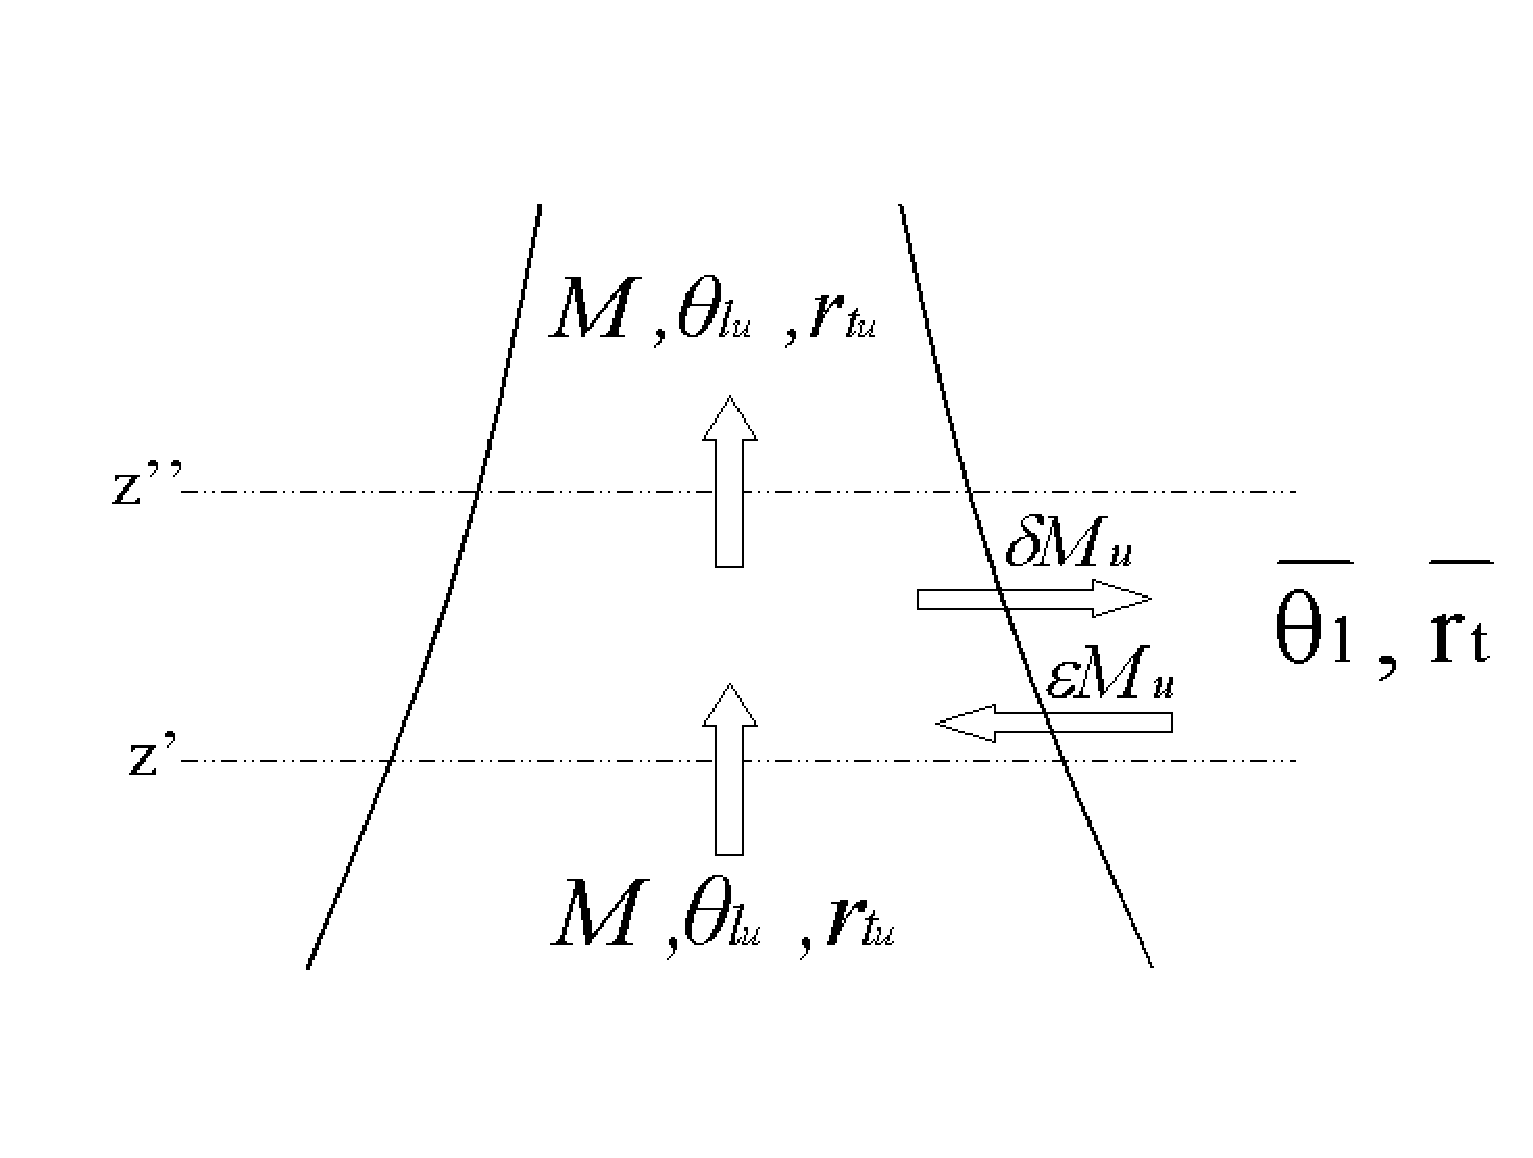
\includegraphics[width=7.5cm]{\EPSDIR/edkfscheme_v3.eps}
	\end{center}
	\caption{Variations of the updraft characteristics $M_u$, $\theta_{lu}$ and $r_{tu}$ and dependent on the mixing with the environment dictated by the entrainment $\epsilon M_u$ and the detrainment $\delta M_u$.}
	\label{fig:SchemeDes}
\end{figure}

The evolution of a conserved parcel characteristic $\phi_u$ during the ascent is defined as in Siebesma (1998):\\
\begin{equation}
\frac{\partial{M_u\phi_u}}{\partial{z}}=E\overline{\phi}-D\phi_u
\label{eq:Phievol1}
\end{equation}
using (\ref{eq:MFevol}) and simplified as:
\begin{equation}
\frac{\partial{\phi_u}}{\partial{z}}=-\epsilon(\phi_u-\overline{\phi})
\label{eq:Phievol2}
\end{equation}
where $\phi_u$ and $\overline{\phi}$ are respectively an updraft conserved variable and its mean value on the grid. This equation is used to determine the evolution of updraft conservative variables such as the liquid potential temperature $\theta_{lu}$ and the total mixing ratio $r_{tu}$ during ascent.

The vertical velocity ($w_u$) equation for the updraft is given by:
\begin{equation}
{w_u}\frac{\partial{w_u}}{\partial{z}}=B_u-\epsilon w_u^2 -P
\label{eq:WevolwithP}
\end{equation}
where on the right-hand side (rhs), the first term is the buoyancy, the second term is the entrainment, and
P represents the pressure term defined in, e.g. numerous studies (Simpson and Wiggert 1969; Siebesma et~al. 2003; Soares et~al. 2004) as a linear combination of the first two terms. Therefore, the equation is simplified as: 
\begin{equation}
w_u\frac{\partial{w_u}}{\partial{z}}=a B_u-b \epsilon w_u^2 
\label{eq:wevol1}
\end{equation}
where $a=1$ and $b=1$, defined respectively as a virtual mass coefficient and a drag coefficient (Simpson and Wiggert 1969). Numerical aspects are given in Appendix \ref{sec:annexe_w}. 

Using the definition of the mass flux, Soares et~al. (2004) and Siebesma et~al. (2007) were able to compute directly the mass flux in the dry portion of their updraft from the vertical velocity obtained from (\ref{eq:wevol1}) and using a constant fraction area. At cloud base, they used a constant value of the cloud fractional area to compute the mass flux and to close the scheme.

Equation (\ref{eq:wevol1}) is used to define the top of the updraft where $w_{u}$ vanishes but also to diagnose the updraft fraction area, $a_u$, which is not a constant or a closure of the scheme as in Soares et~al. (2004) and Siebesma et~al. (2007). 

Thanks to the independent computations of both mass flux $M_u$ (\ref{eq:MFevol}) and $w_{u}$ (\ref{eq:wevol1}), the updraft fraction area can vary vertically, and is defined as
\begin{equation}
   a_u=\frac{M_u}{\rho w_u}.
   \label{eq:updraft_fraction}
\end{equation}
The vertical variations of this last variable are important because $a_u$ is used to diagnose the cloud fraction (see next section).

The mass flux approach is also used to realize a non-local mixing of momentum along the vertical in addition to the mixing yet realized by the turbulent scheme via the eddy-diffusivity approach. But, since the momentum is not conservative, the effect of pressure perturbations is added using a parameterization from Gregory et~al. (1997). The evolution of the updraft horizontal wind component is defined as: 
%\begin{eqnarray}
\begin{equation}
    \frac{\partial{u_u}}{\partial{z}}=-\epsilon(u_u-\overline{u})+C_u\frac{\partial{\overline{u}}}{\partial{z}}\\
\label{eq:uevol},
\end{equation}
\begin{equation}
    \frac{\partial{v_u}}{\partial{z}}=-\epsilon(v_u-\overline{v})+C_v\frac{\partial{\overline{v}}}{\partial{z}}
\label{eq:uevol1},
\end{equation}
where $C_u=C_v=0.5$, and $u_u$ ($v_u$) represents the zonal (meridional) component of wind modified during the ascent in the updraft; $\overline{u}$ and $\overline{v}$ are zonal and meridional mean wind components respectively. 

\subsection{Lateral mass exchanges}

The definition of entrainment and detrainment is the crucial issue in this type of parameterization. Various studies have used different definitions for various PBL regimes (e.g., Siebesma 1998; Neggers et~al. 2002; De~Rooy and Siebesma 2008).

We have chosen to define lateral mass exchanges from physical characteristics of the CBL. Arakawa (2004) explained that buoyancy is an important parameter in shallow convection. Moreover, the vertical velocity $w_u$ is considered as a pertinent parameter in the description of mixing between dry updraft or the cloud and their environment in shallow convection. Neggers et~al. (2002) defined the entrainment as inversely proportional to vertical velocity for shallow cumulus convection, and Cheinet (2003) also applies this formulation to dry plumes. This means that $\epsilon$ is not constant but decreases with higher vertical velocities. In other terms, an updraft with strong vertical velocity will be isolated from its environment. 

In the dry portion of the CBL, $\epsilon$ and $\delta$ take into account physical characteristics of a buoyant ascending parcel. Equation (\ref{eq:wevol1}) shows that buoyancy is linked to vertical velocity, ${w_u}^2$ being a vertical integral of the buoyancy. However, locally, both can be independent, for example in the non-buoyant part where negative buoyant air can still be ascending. Young (1988) explained that the correlation between buoyancy and $w$ decreases in the upper part of the CBL, the buoyancy acting as a displacing force in the lower part of the CBL and as a restoring force in the upper part of the CBL. Thus, lateral mixing does not only depend on the vertical velocity as in Neggers et~al. (2002) but must be locally defined as an equilibrium between $w_u$ and buoyancy $B_u$. By dimensional analysis (Buckingham 1914), we obtain:
\begin{equation}
\epsilon_{dry},\delta_{dry} \propto \frac{B_u}{w_u^2} 
\label{eq:ent_delt_BW}
\end{equation}
where $B_u=g(\theta_{v,u}-\overline{\theta_v})/\overline{\theta_v}$ is the buoyancy of the air parcels in the updraft.

Near the ground, a relative strong buoyancy and a weak vertical velocity allow strong entrainment to import many air parcels in the updraft, implying a positive proportionality coefficient for $\epsilon$. Near the inversion, in the non-buoyant zone, much air is detrained implying a negative proportionality coefficient for $\delta$. Since entrainment and detrainment rates cannot be negative, the entrainment rate is zero where the updraft is non-buoyant compared to its surrounding environment. Conditional sampling of detrainment in LES has shown that detrainment is not null in the mixed layer (see Fig. 9c of Pergaud et~al. (2009)), so to keep a positive detrainment in the buoyant part of the updraft, a minimum detrainment is defined using a modified formulation from Lappen and Randall (2001): $\delta=(L_{up}-z)^{-1}$. 

Eventually, in the dry portion of the CBL, entrainment and detrainment are defined as:
\begin{eqnarray}
\epsilon_{dry} = Max\left[0,C_{\epsilon} \frac{B_u}{w_u^2} \right],  \\
\delta_{dry} = Max\left[\frac{1}{L_{up}-z}, C_{\delta} \frac{B_u}{w_u^2} \right],
\label{eq:eps_ent_delt}
\end{eqnarray}
where $L_{up}$ is the Bougeault and Lacarr\`ere (1989) (BL89) upward mixing length, $C_{\delta}$ and $C_{\epsilon}$ have been tuned to fit one-dimensional (1D) entrainment and detrainment to LES, $C_{\delta}=-10$ and $C_{\epsilon}=0.55$. Numerical aspects are given in Appendix \ref{sec:annexe_e}. 

In the cloudy part, several descriptions of the exchanges exist. 

We have chosen to define two different types of exchange differentiating the dry portion of the updraft from the moist one due to the fact that the environment of any updraft is strongly turbulent compared to the environment of a cloud. 
Taylor and Baker (1991) have emphasized the importance of buoyancy sorting in determining the cloud composition and in defining a continued lateral entrainment and detrainment. Zhao and Austin (2003) explained that a buoyancy sorting model can be used as a physically more realistic alternative to entraining plume models in shallow cumulus convection resolving notably the Warner paradox. In the parameterization presented here, if the lifting condensation level (LCL) is reached, lateral exchanges are computed using the parcel buoyancy sorting approach of Kain and Fritsch (1990) (KF90 in the following). Details are given in Kain and Fritsch (1990) and Bechtold et al. (2001) and you can see the chapter dealing with the Kain-Fritsch-Bechtold convection scheme.
However, minor modifications have been put in the EDKF parameterization, the new parameterization uses a uniform distribution of the air parcels although, in the original formulation, the distribution was Gaussian. 

\subsection{Scheme initialization and closure}

Since the scheme is integrated upward from the surface (level $z_{grd}$), $M_u(z_{grd})$ is computed as a function of $w_*$ as in Grant (2001) but at the surface, contrary to the closure at the cloud base defined by Grant (2001),
\begin{equation}
M_{u}(z_{grd})=C_{M_0}\rho(\frac{g}{\overline{\theta_{vref}}}\overline{{w'\theta_{v}'}_s} L_{up})^{1/3}
\label{eq:MFz0}
\end{equation}
where $\overline{{w'\theta_{v}'}_s}$ is the surface buoyancy flux, ${L_{up}}$ is the BL89 upward mixing length corresponding to the distance that a parcel leaving the ground travel due to buoyancy. The value of $C_{M_0}=0.065$ is based on LES results according to Pergaud et~al. (2009). Note that, in the surface layer, this value is larger than the value $C_{M_0}=0.03$ originally proposed by Grant (2001) at the LCL. 

The rising parcel characteristics are determined at the ground using the formulation of Soares et~al. (2004) in which an excess is added to the environmental values. For example, the updraft liquid potential temperature near the ground is:
\begin{equation}
\theta_{lu}(z_{grd})=\overline{\theta_l}(z_{grd})+\alpha\frac{{\overline{w'\theta_l'}}_s}{e^{1/2}(z_{grd})}
\label{eq:Phiz0}
\end{equation}
where the value of $\alpha$ is $0.3$ as in Soares et~al. (2004). Sensitivity tests in the range [0,1] indicate that results are independent of $\alpha$. This excess is formulated as a function of the surface-layer variability according to Troen and Mahrt (1986) who demonstrated that the excess is well correlated with the ratio of the surface heat flux and the square root of turbulent kinetic energy. A similar equation is used for $r_t$. 

At the surface, $w_u$ is initialized from the turbulent kinetic energy $e$ (provided by the turbulence scheme),
\begin{equation}
  {w_u}^2(z_{grd})=\frac{2}{3}e(z_{grd}).
  \label{Wz0}
\end{equation}

\subsection{The subgrid condensation scheme}

The updraft scheme represents the dynamical evolution of an air parcel during its ascent. Condensation can occur within the parcel. Therefore, a diagnostic sub-grid cloud based on the updraft characteristics is added. Although conservative variables are used, we can diagnose a sub-grid liquid mixing ratio $r_{c_{up}}$ and a cloud fraction $CF$. $r_{c_{up}}$ is computed from $\theta_l$, $r_t$ and pressure using a variation of all or nothing scheme since the updraft air parcels are considered completely cloudy.
$CF$ is defined proportional to the updraft fraction on the grid $a_u$:
\begin{equation}
  CF=C_{cf} * a_u
  \label{eq:CloudFrac}
\end{equation}
where $C_{cf}=2.5$. The horizontal size of the cloud is 2.5 times the size of the updraft. This parameter has been tuned to fit the 1D cloud fraction to LES results. This coefficient represents the difference between cloudy core fraction and cloud fraction.

The liquid mixing ratio can be approximated by the product between the cloud fraction previously computed and the updraft liquid mixing ratio computed from the updraft conservative variables (Bechtold and Cuijpers 1995):
\begin{equation}
  \overline{r_c}= CF * r_{c_{up}}
\label{eq:RcFrac}
\end{equation}

In our parameterization, $r_c$ is not a prognostic variable. If the mass flux becomes null, the cloud disappears totally. Only a prognostic cloud scheme can evaporate a cloud over several timesteps. So passive clouds that are not maintained by a thermal are not taken into account in the parameterization. However, here, $\overline{r_c}$ represents only the contribution of the shallow convection clouds. Others contributions for clouds can come from the subgrid turbulence scheme or from microphysics scheme (notably for resolved clouds). 

\section{Initialisation of Mass-Flux scheme at hectometric scales}

The triggering controls the activation of the mass-flux scheme at the surface while the closure controls its intensity. Often the boundary-layer mass-flux scheme triggers as soon as the surface sensible heat flux is positive while the intensity of the mass-flux at the ground is proportional to the convective velocity scale (see Pergaud et~al.,2009). 

Firstly, concerning the closure, Figure~\ref{trigDavid}a shows the subgrid mass-flux normalized by the convective velocity scale as a function of the normalized resolution in the IHOP case at $1200$ LT and the ARM case at $1400$ LT in the middle of the boundary layer. The mass-flux normalized by the convective velocity scale in both the IHOP and ARM cases is dependent on the resolution normalized by the height of the thermals : it is constant at mesoscales and larger than in LES. Here the mass flux is computed in the middle of the CBL. It cannot be diagnosed directly at the ground where there is no really thermal formed yet and where the turbulent is more strongly dependent on the subgrid turbulence scheme. The normalized mass flux as a function of the normalized resolution has the same shape at all altitudes in the boundary layer (not shown). Therefore, here we propose to make the constant of proportionality between the mass-flux at the ground and the convective velocity scale (computed at ground level for the whole domain, $w*$) dependent on the resolution by this function :

\begin{equation}
	\sigma(\frac{M_u}{w_*})=tanh(C\times\sqrt(\Delta x \times \Delta y)/L_{up})
\label{eq:MuHect}
\end{equation}
In the magenta fit plotted in Fig.~\ref{trigDavid}a, $C=1.83$. We propose to use this function in the parametrization in order to make it scale-aware.

Moreover, the subgrid mass-flux variability is larger in the grey zone than in the LES and at mesoscales. This is visible in Fig.~\ref{trigDavid}b which shows the standard deviation of the mass-flux normalized by the convective velocity scale ($\sigma(\frac{M_u}{w*})$) as a function of the normalized resolution in the IHOP case at $1200$~LT and the ARM case at $1400$~LT in the middle of the CBL. The large variability in the grey zone is also visible on the buoyancy and the entrainment (cf.~Honnert et al.,2016) and it is consistent with Dorrestijn et al. (2013) which showed that the heat flux variability is larger in the grey zone. The fit of the data of Fig.~\ref{trigDavid}b is:

\begin{figure}
\subfigure[\large Distribution]{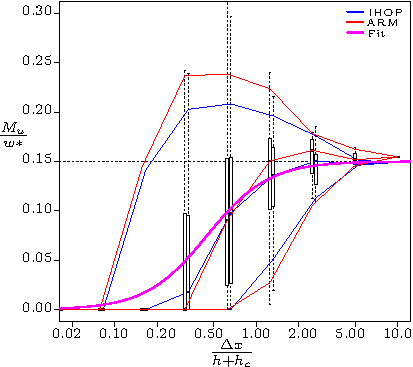
\includegraphics[width=0.45\textwidth]{EPS/MU_dx_fit_REVIEW}}
\subfigure[\large Dispersion]{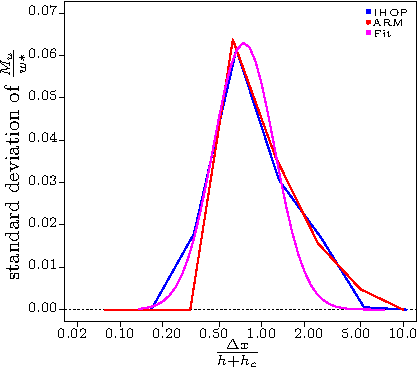
\includegraphics[width=0.45\textwidth]{EPS/dispersion_Mu_REVIEW}}
\caption[]{(a) Mass-flux of the subgrid thermals normalized by the convective velocity scale for grid cells ranging from $250$~m to $8$~km in the middle of the boundary layers of the ARM case at $1400$ LT (blue points) and the IHOP case at $1200$ LT (red points) as a function of $\Delta x/({h}+{h}_{c})$. Boxplots of the data (one per case) : the box shows 50\% of the data and the line 99.3\%. Median, quantile 5\% and 95\% in (red and blue) lines. A fit of the data (see text for more details) is in magenta. (b) Standard deviation of the same data in the same colors as in (a) as a function of the normalized horizontal resolution.}
\label{trigDavid}
\end{figure}

Concequently, the closure of the mass-flux scheme of Pergaud et~al. (2009) at hectometric scales depend on the model resolution following Eq.~\ref{eq:MuHect}.   

\section{Appendix}
\subsection{Mass flux in the surface layer compared to $w_*$}
\label{sec:MF_W}

The mass flux near the surface has been set proportional to the convective vertical velocity scale $w_*$ as in Grant (2001). The coefficient of proportionality $C_{M_0}$ in our scheme cannot have the same value than the one used by Grant (2001) due to the fact that Grant (2001) defines this relation at the LCL. So we used the CS defined in Pergaud et~al. (2009) to obtain mass flux values in the surface layer for different convective cases at different dates (IHOP, ARM).

\begin{figure}
 \begin{center}
		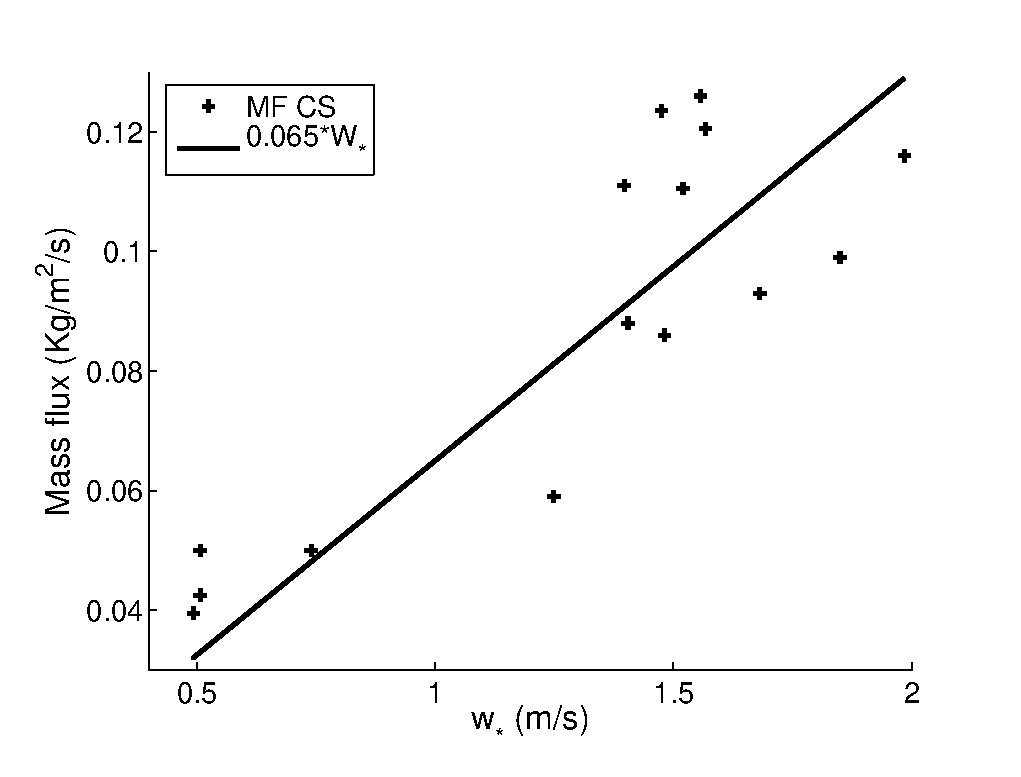
\includegraphics[width=9cm]{\EPSDIR/edkfMF_F_W.eps}
	\end{center}
	\caption{Mass flux in the surface layer computed using the Conditionnal Sampling defined in Pergaud et~al. (2009) versus sub-cloud layer velocity scale $w_*$. Line shows $M=0.065w_*$.}
	\label{fig:MF_F_W}
\end{figure}

Figure \ref{fig:MF_F_W} is a plot of the surface layer mass flux against sub-cloud layer velocity scale. The LES data suggest that $C_{M_0}=0.065$.

\subsection{Analytical solution for the vertical velocity $w_u$}
\label{sec:annexe_w}
Equation (\ref{eq:wevol1}) presents the computation for vertical velocity in the updraft $w_u$. Combining the equation for entrainment (\ref{eq:eps_ent_delt}), the $w_u$ equation becomes :
\begin{equation}
   \frac{\partial{{w_u}^2}} {\partial{z}}=2 a B_u-2 b C_{\epsilon}max(0,B_u)
\label{eq:wevol2}
\end{equation}
$C_{BUO}$ is defined equal to $2a$ if $B_u<0$ (entrainment is zero) and to $2(a-bC_{\epsilon})$ if $B_u>0$.
This equation is integrated over each layer. Figure \ref{fig:SchemeDes2} presents this integral. If $z'$ is layer bottom, $z''$ is layer top and $\Delta z_D = z''-z'$,  ${w_u}^2$ is defined by:

\begin{eqnarray}
   \int_{\Delta z_D}\frac{\partial{{w_u}^2}}{\partial{z}}dz=\int_{\Delta z_D} C_{BUO} B_u dz\\
   {w_u}^2(z'')-{w_u}^2(z')= C_{BUO}\frac{g}{\theta_{ref}}\int_{\Delta z_D} \left[    \theta_{v_{up}}(z)-\overline{\theta_v}(z)\right]  dz
   \label{eq:primitive1}
\end{eqnarray}

$\theta_{vup}$ is assumed constant between $z'$ and $z''$, and the variations of $\overline{\theta_v}$ is supposed linear between z' and z''.
\begin{eqnarray}
   \overline{\theta_v}(z)= \alpha_1 z + \overline{\theta_v}(z')\\
   \theta_{v_{up}}(z)    = \theta_{v_{up}}(z')
   \label{eq:fonction_lineaire}
\end{eqnarray}
So the integral for $w_u$ becomes
\begin{equation}
   {w_u}^2(z'') - {w_u}^2(z')= C_{BUO}\frac{g}{\theta_{ref}}\int_{\Delta z_D} \left[- \alpha_1z - \overline{\theta_v}(z') + \theta_{v_{up}}(z')\right]  dz \\
   \label{eq:primitive2}
\end{equation}

After computation, $w_u$ at the level $z''$ computed from the level $z'$ is :
\begin{equation}
   {w_u}^2(z'')= C_{BUO}\frac{g}{\theta_{ref}} \Delta z_D(\frac{ - \alpha_1}{2}\Delta z_D - \overline{\theta_v}(z') + \theta_{v_{up}}(z')) + {w_u}^2(z') 
   \label{eq:primitive3}
\end{equation}


\subsection{Analytical integrated solution for entrainment and detrainment}
\label{sec:annexe_e}

The entrainment $\epsilon$ is defined by equation (\ref{eq:eps_ent_delt}). This equation is integrated, as for $w_u$, on each vertical grid size for example between $z'$ and $z''$ (see on Fig. \ref{fig:SchemeDes2}):
\begin{equation}
   \epsilon = \frac{C_{\epsilon}}{\Delta z_D}\int_{\Delta z_D} \frac{B}{{w_u}^2}dz\\
   \label{eq:primitive4}
\end{equation}
Using (\ref{eq:primitive3}), $\epsilon$ becomes
\begin{eqnarray}
   \epsilon = \frac{C_{\epsilon}g}{\Delta z_D \theta_{ref}}\int_{\Delta z_D} \frac{ \theta_{v_{up}}(z') - \alpha_1 z +  \overline{\theta_v}(z')} {C_{BUO}\frac{g}{\theta_{ref}} z( - \alpha_1 z - \overline{\theta_v}(z') + \theta_{v_{up}}(z')) + {w_u}^2(z')}dz\\
   \epsilon = \frac{C_{\epsilon}}{\Delta z_D C_{BUO}}\int_{\Delta z_D} \frac{- \alpha_1 z + \theta_{v_{up}}(z') +  \overline{\theta_v}(z')} { \frac{- \alpha_1}{2}z^2 - \overline{\theta_v}(z')z + \theta_{v_{up}}(z')z) + \frac{\theta_{ref} {w_u}^2(z')} {g C_{BUO}}}dz.
   \label{eq:primitive5}
\end{eqnarray}

noting $X=\frac{- \alpha_1}{2}z^2 - \overline{\theta_v}(z')z + \theta_{v_{up}}(z')z) + \frac{\theta_{ref}{w_u}^2(z')}{gC_{BUO}}$:

\begin{eqnarray}
   dX= ((- \alpha_1) z + \theta_{v_{up}}(z') +  \overline{\theta_v}(z'))dz\\
   \epsilon = \frac{C_{\epsilon}}{C_{BUO}\Delta z_D}\int_{\Delta z_D} \frac{dX}{X}\\
   \epsilon = \frac{C_{\epsilon}}{C_{BUO}\Delta z_D}[Ln(X)]_{\Delta z_D}
   \label{eq:primitive6}
\end{eqnarray}

After computation, $\epsilon$ is defined as :
\begin{equation}
   \epsilon=\frac{C_{\epsilon}}{C_{BUO}\Delta z_D} ln\left[ 1+\frac{C_{BUO}\Delta z_D}{{w_u}^2(z')\theta_{ref}} (\frac{- \alpha_1}{2} \Delta z - \theta_{v_{up}}(z') +  \overline{\theta_v}(z'))\right]\\
   \label{eq:epsilon}
\end{equation}
where $\alpha_1$ is defined as previously. An identical solution can be found for $\delta$ taking the absolute value of the buoyancy.

A formulation of the transition between cloudy and dry regime is added to limit the sensitivity of the scheme to the change in the computation of entrainment and detrainment. If a liquid mixing ratio is detected at z'' using an "all or nothing" adjustment from updraft variables, the LCL height is determined assuming a linear increase of $r_c$ with height. A weight for the KF90 lateral exchanges is defined proportional to the cloudy part occupying grid and integral dry entrainment and detrainment are computed only on the height of the dry part.

\begin{figure}
  \begin{center}
    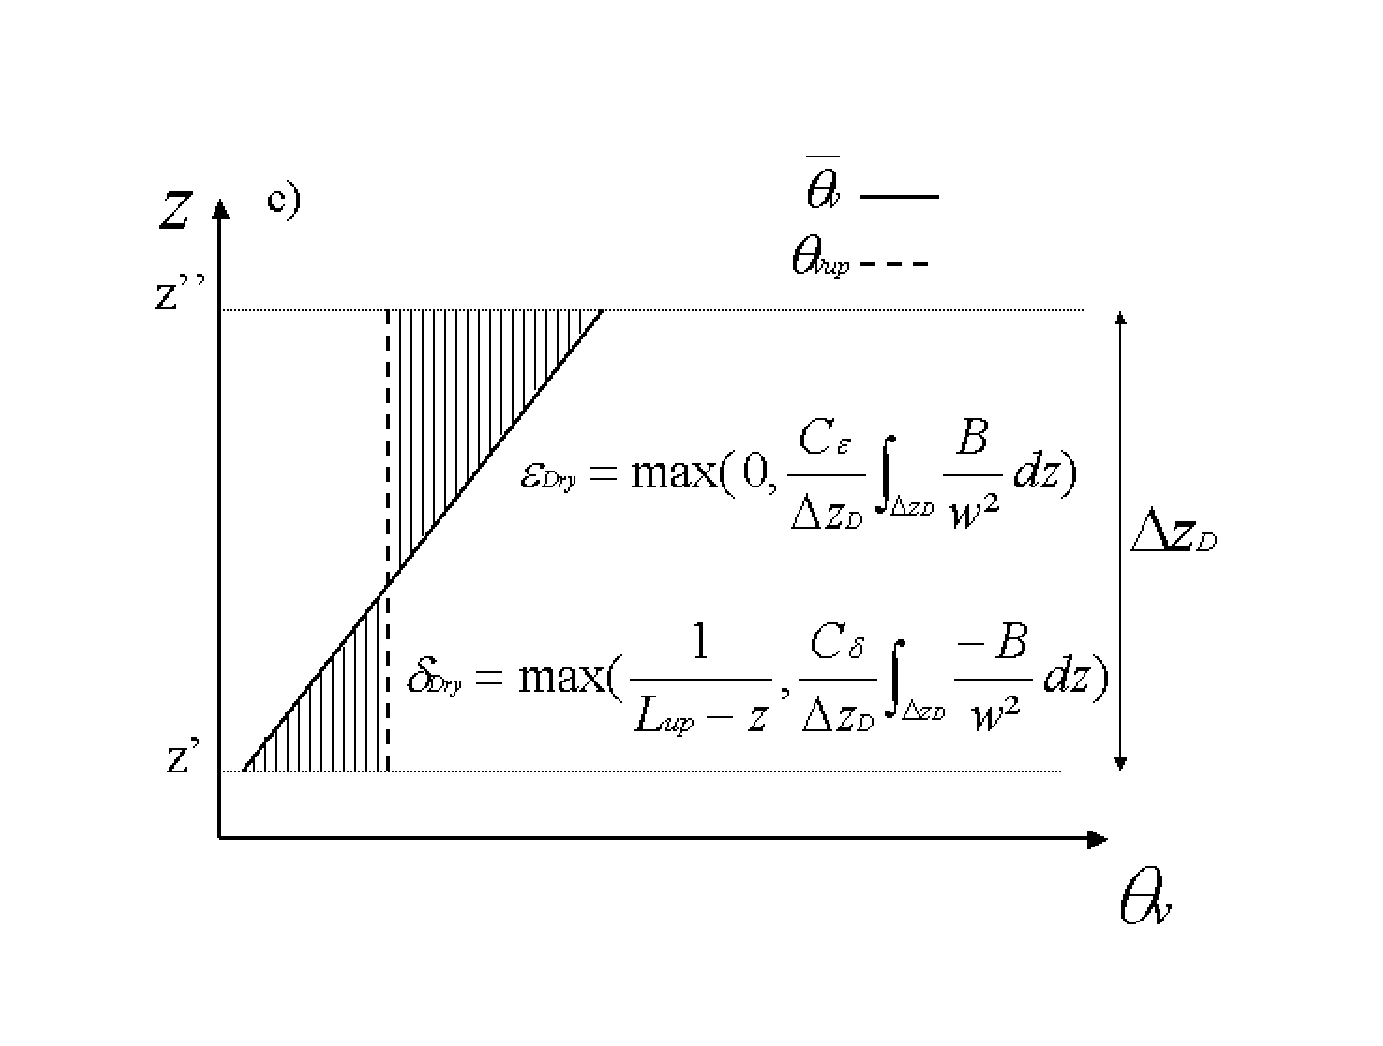
\includegraphics[width=11cm]{\EPSDIR/edkfTHL_DRY_PWT_v2.eps}
  \end{center}
  \caption{Parameterized entrainment and detrainment for dry layer}
  \label{fig:SchemeDes2}
\end{figure}

\section{References}

\noindent \por
Arakawa, A., 2004: 
The Cumulus Parameterization Problem: Past, Present, and Future.
{\it J. Clim.}, {\bf 17}, 2493--2525.

\noindent \por
Bechtold, P., and~ J. W. M. Cuijpers, 1995:
Cloud perturbations of temperature and humidity: A LES study.
{\it Bound. Layer. Meteor.}, {\bf 76}, 377--386.

\noindent \por
Bechtold, P., E. Bazile, P. Mascart and E. Richard, 2001:
A Mass flux convection scheme for regional and global models.
{\it Quart. J. Roy. Meteor. Soc.}, {\bf 127}, 869-886.

\noindent \por
Bougeault, P, and P. Lacarr\`ere, 1989: Parameterization of Orography-Induced
  Turbulence in a Mesobeta-Scale Model.
{\it Mon. Wea. Rev.}, {\bf 117}, 1872--1890.

\noindent \por
Buckingham, E., 1914: On physically similar systems: Illustrations of the use of
  dimensional equations.
{\it Phys. Rev.}, {\bf IV}, 345--376.

\noindent \por
Cheinet, S., 2003: A multiple Mass-Flux Parameterization for the
  Surface-Generated Convection. Part1: Dry Plumes.
{\it J. Atmos. Sci.}, {\bf 60}, 2313--2327.

\noindent \por
Cuxart, J., P. Bougeault, and J.-L. Redelsperger, 2000:
A turbulence scheme allowing for mesoscale and large-eddy simulations.
{\it Quart. J. Roy. Meteor. Soc.}, {\bf 126,} 1--30.

\noindent \por
De~Rooy, W. C., and P. Siebesma, 2008:
 A simple parameterization for detrainment in shallow cumulus.
{\it Mon. Wea. Rev.}, {\bf 136}, 560--576.

\noindent \por
Dorrestijn J, Crommelin DT, Siebesma AP and Jonker HJJ, 2013:
Stochastic convection parametrization estimated from high-resolution model data.  27:133--148
{\it Theor Comput Fluid Dyn}, {\bf 27}, 133--148.

\noindent \por
Grant, A. L. M., 2001: Cloud-base fluxes in the cumulus-capped boundary layer.
{\it Quart. J. Roy. Meteor. Soc.}, {\bf 127}, 407--421.

\noindent \por
Gregory, D., R. Kershaw, and P. M. Inness, 1997:
 Parametrization of momentum transport by
  convection. II: Tests in single-column and general circulation models.
{\it Quart. J. Roy. Meteor. Soc.}, {\bf 123}, 1153--1183.

\noindent \por
Honnert, R., Couvreux, F., Masson, V. et David Lancz, 2016 :
Sampling the Structure of Convective Turbulence and Implications for Grey-Zone Parametrizations
{\it Bound. Layer. Meteor.}, {\bf 160}, 133.

\noindent \por
Hourdin, F., F. Couvreux, and L. Menut, 2002:
 Parameterization of the Dry Convective
  Boundary Layer Based on a Mass Flux Representation of Thermals.
{\it J. Atmos. Sci.}, {\bf 59}, 1105--1122.

\noindent \por
Kain, J. S., and J. M. Fritsch, 1990: A one-dimensional
entraining/detraining plume model and its application in
convective parameterizations. {\it J. Atmos. Sci.},
{\bf 47}, 2784-2802.

\noindent \por
Lappen, C. L., and D. A. Randall, 2001:
Toward a Unified Parameterization of the Boundary Layer and Moist Convection. 
Part2 : Lateral Mass Exchanges and Subplume-Scale Fluxes.
{\it J. Atmos. Sci.}, {\bf 58}, 2037--2051.

\noindent \por
Neggers, R. A. J., P. Siebesma, and H. J. J. Jonker, 2002:
 A Multiparcel Model for Shallow Cumulus Convection.
{\it J. Atmos. Sci.}, {\bf 59}, 1655--1668.

\noindent \por
Pergaud, J., V. Masson, S. Malardel, and F. Couvreux, 2009:
A Parameterization of Dry
  Thermals and Shallow Cumuli for Mesoscale Numerical Weather Prediction.
{\it Bound. Layer. Meteor.}, {\bf 132}, 83--106.

\noindent \por
Siebesma, P., 1998: Shallow Cumulus Convection.
In {\it "Buoyant convection in geophysical flows"} (Eds. E.J. Plate et al),
441--486.

\noindent \por
Siebesma, P., C. S. Bretherton, A. Brown, A. Chlond, J. Cuxart, 
P. G. Duynkerke, H. Jiang, M. Khairoutdinov, D. Lewellen, C. H. Moeng,
E. Sanchez, B. Stevens, and D. E. Stevens, 2003:
A Large Eddy Simulation Intercomparaison Study of Shallow Cumulus Convection.
{\it J. Atmos. Sci.}, {\bf 60}, 1201--1219.

\noindent \por
Siebesma, P., P. M. M. Soares, and J. Teixeira, 2007:
A combined Eddy-Diffusivity Mass-Flux 
approach for the convective boundary layer.
{\it J. Atmos. Sci.}, {\bf 64}, 1230--1248.

\noindent \por
Simpson J, and V. Wiggert, 1969: Models of precipitating cumulus towers.
{\it Mon. Wea. Rev.}, {\bf 97}, 471--489.

\noindent \por
Soares, P. M. M., P. M. A. Miranda, A. P. Siebesma, and J. Teixeira, 2004:
An Eddy-Diffusivity/Mass-Flux parameterization for dry and shallow cumulus
  convection.
{\it Quart. J. Roy. Meteor. Soc.}, {\bf 130}, 3055--3079.

\noindent \por
Taylor, G. R., and M. B. Baker, 1991: 
Entrainment and Detrainment in cumulus clouds.
{\it J. Atmos. Sci.}, {\bf 48}, 112--121.

\noindent \por
Troen, I. B., and L. Mahrt, 1986:
A simple model of the atmospheric boundary layer: 
Sensitivity to surface evaporation.
{\it Bound. Layer. Meteor}, {\bf 37}, 129--148.

\noindent \por
Young, G. S., 1988: Turbulence Structure of the convective Boundary Layer. Part II:
  Phoenix 78 Aircraft Observations of Thermals and their environment.
{\it J. Atmos. Sci.}, {\bf 45}, 727--735.

\noindent \por
Zhao, M., and P. H. Austin, 2003:
Episodic Mixing and Buoyancy-Sorting Representations
  of Shallow Convection: A Diagnostic Study.
{\it J. Atmos. Sci.}, {\bf 60}, 892--912.
